% ==========================================
% INTEGRALI DI SUPERFICIE DI I SPECIE
% ==========================================
\usetikzlibrary{calc, arrows.meta, positioning, 3d}

\chapter{Integrali di superficie di 1ª specie}

\section{Rappresentazione delle Superfici}

\subsection{Forma parametrica}
Data una superficie bidimensionale in uno spazio tridimensionale, se definiamo i parametri $u$ e $v$ in un dominio $D$, l'immagine del dominio sarà una superficie $\Sigma$ nello spazio 3D descritta dalla funzione vettoriale:
\begin{equation}
    \vec{r}(u,v) = \begin{pmatrix} x(u,v) \\ y(u,v) \\ z(u,v) \end{pmatrix} \quad \text{con } (u,v) \in D
\end{equation}



\subsection{Esempio: La sfera in forma parametrica}
Sfruttando latitudine e longitudine, la sfera di raggio $R$ si parametrizza come:
$$ x = R \cos\theta \cos\phi $$
$$ y = R \cos\theta \sin\phi $$
$$ z = R \sin\theta $$
dove $\theta \in \left[-\frac{\pi}{2}, \frac{\pi}{2}\right]$ (latitudine) e $\phi \in [0, 2\pi]$ (longitudine).

\begin{figure}[H]
    \centering
    \begin{tikzpicture}[scale=1]

        % ==========================================
        % PARTE SINISTRA: Dominio 2D (Piano uv)
        % ==========================================
        
        % Assi u e v
        \draw[thick, ->] (0,0) -- (4,0) node[below] {$u$};
        \draw[thick, ->] (0,0) -- (0,3.5) node[left] {$v$};

        % Regione D (curva chiusa smussata)
        \draw[red, thick] plot [smooth cycle, tension=0.7] coordinates {
            (1, 1)
            (2.2, 1.2)
            (2.5, 0.8) % Piccola rientranza in basso come nel disegno
            (3.2, 1.5)
            (2.8, 2.5)
            (1.5, 2.6)
            (0.8, 1.8)
        };
        % Etichetta D
        \node[red, font=\Large] at (2, 1.8) {$D$};


        % ==========================================
        % CENTRO: Freccia di mappatura
        % ==========================================
        
        % Freccia curva con l'etichetta del vettore r
        \draw[->, thick] (3.8, 2) to[out=15, in=165] node[above, font=\large] {$\vec{r}$} (6.2, 2);


        % ==========================================
        % PARTE DESTRA: Superficie 3D
        % ==========================================
        
        % Spostiamo l'origine per la parte 3D
        \begin{scope}[shift={(7,0)}]
            
            % Assi 3D (x, y, z)
            \draw[thick] (0,0) -- (-0.8,-2); % Asse uscente dallo schermo
            \draw[thick] (0,0) -- (4.5,0);   % Asse orizzontale
            \draw[thick] (0,0) -- (0,3.5);   % Asse verticale

            % Regione S (curva chiusa smussata)
            \draw[red, thick] plot [smooth cycle, tension=0.7] coordinates {
                (1.5, 1)
                (2.5, 0.7)
                (3.6, 1.1)
                (3.5, 2.2)
                (2.8, 3)
                (1.2, 2.5)
                (0.8, 1.8)
                (1.4, 1.5) % Piccola rientranza a sinistra
            };
            % Etichetta S
            \node[red, font=\Large] at (2.4, 1.9) {$S$};
            
        \end{scope}

    \end{tikzpicture}
    \caption{Mappatura di un dominio $D$ in una superficie $S$ tramite $\vec{r}(u,v)$.}
\end{figure}

\newpage
\subsection{Superficie come grafico di una funzione}
Molto spesso una superficie può essere vista come il grafico di una funzione a due variabili, espressa come l'insieme dei punti $(x, y, f(x,y))$, dove il dominio $D$ giace nel piano $xy$.

\begin{figure}[H]
    \centering
    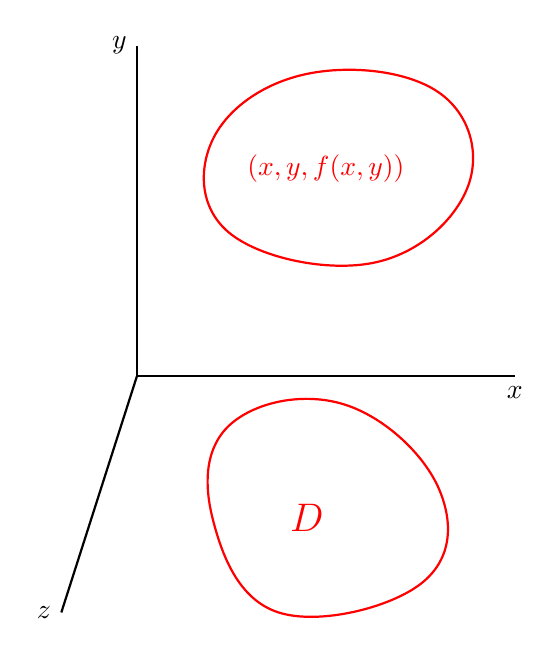
\begin{tikzpicture}[scale=1.2] % Aumentato leggermente per fare spazio al testo

        % ==========================================
        % ASSI CARTESIANI
        % ==========================================
        
        % Asse x (orizzontale a destra)
        \draw[thick] (0,0) -- (4,0) node[below] {$x$};
        
        % Asse y (verticale in alto)
        \draw[thick] (0,0) -- (0,3.5) node[left] {$y$};
        
        % Asse z (diagonale uscente verso il basso a sinistra)
        \draw[thick] (0,0) -- (-0.8,-2.5) node[left] {$z$};


        % ==========================================
        % DOMINIO INFERIORE (D)
        % ==========================================
        
        % Forma irregolare rossa in basso (nel piano xz)
        \draw[red, thick] plot [smooth cycle, tension=0.7] coordinates {
            (1, -0.5)
            (2.2, -0.3)
            (3.2, -1.2)
            (3, -2.2)
            (1.5, -2.5)
            (0.8, -1.5)
        };
        % Etichetta D
        \node[red, font=\Large] at (1.8, -1.5) {$D$};


        % ==========================================
        % SUPERFICIE SUPERIORE (x, y, f(x,y))
        % ==========================================
        
        % Forma irregolare rossa in alto
        \draw[red, thick] plot [smooth cycle, tension=0.7] coordinates {
            (1, 1.5)
            (2.5, 1.2)
            (3.5, 2)
            (3.2, 3)
            (1.8, 3.2)
            (0.8, 2.5)
        };
        % Etichetta (x, y, f(x,y))
        \node[red, font=\normalsize] at (2, 2.2) {$(x, y, f(x,y))$};

        % Linee di collegamento opzionali (se in futuro vorrai aggiungere linee 
        % tratteggiate per mostrare la proiezione, puoi farlo qui)
        % \draw[dashed, gray] (1.8, -1.5) -- (2, 2.2);

    \end{tikzpicture}
    \caption{Rappresentazione di una superficie sopra un dominio $D$.}
\end{figure}

\subsection{Esempio: La sfera come grafico di funzione}
Dall'equazione cartesiana della sfera $x^2 + y^2 + z^2 = R^2$, possiamo isolare la $z$ ottenendo due funzioni distinte:
\begin{itemize}
    \item L'emisfero superiore: $f(x,y) = \sqrt{R^2 - x^2 - y^2}$
    \item L'emisfero inferiore: $f(x,y) = -\sqrt{R^2 - x^2 - y^2}$
\end{itemize}

\subsection{Superfici di livello (Forma implicita)}
Una superficie può anche essere descritta implicitamente come una \textit{superficie di livello} di una funzione a tre variabili:
$$ F(x,y,z) = c $$
Ad esempio, la sfera di raggio $R$ si può definire implicitamente dall'equazione $F(x,y,z) = x^2 + y^2 + z^2 = R^2$.


\newpage
\section{Integrale di Superficie di 1ª Specie}

\subsection{Costruzione geometrica e approssimazione dell'area}
Consideriamo una superficie $\Sigma$ descritta vettorialmente da $\vec{r}(u,v)$. \\
Se suddividiamo il dominio $D$ nello spazio dei parametri $(u,v)$ attraverso un reticolo, l'immagine di questo dominio si proietterà come un reticolo curvo sulla superficie $\Sigma$ nello spazio 3D. 

\begin{figure}[H]
    \centering
    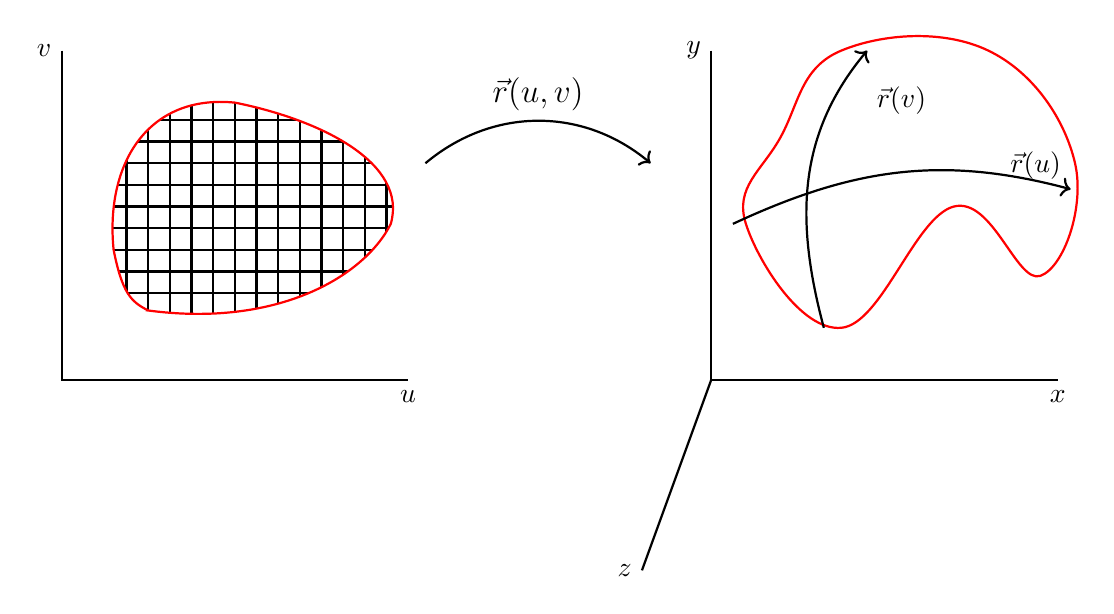
\begin{tikzpicture}[scale=1.1]

        % ==========================================
        % PARTE SINISTRA: Dominio con griglia (Piano uv)
        % ==========================================
        
        % Assi u e v (linee semplici come nel disegno)
        \draw[thick] (0,3.8) node[left] {$v$} -- (0,0) -- (4,0) node[below] {$u$};

        % Definiamo il percorso della regione D per poterlo riutilizzare
        % Questo ci permette di usarlo sia per tagliare la griglia che per disegnare il bordo
        \def\dominio{
            (1, 0.8) .. controls (2.5, 0.6) and (3.5, 1.2) .. 
            (3.8, 1.8) .. controls (4, 2.5) and (3, 3) .. 
            (2, 3.2) .. controls (1, 3.3) and (0.5, 2.5) .. 
            (0.6, 1.5) .. controls (0.7, 1) and (0.8, 0.9) .. cycle
        }

        % Disegniamo la griglia confinata dentro la forma
        \begin{scope}
            % Il comando \clip fa sì che tutto ciò che viene disegnato dopo in questo 'scope'
            % sia visibile solo all'interno del percorso definito.
            \clip \dominio;
            \draw[step=0.25, black, thick] (0,0) grid (4.5, 4);
        \end{scope}

        % Disegniamo il bordo rosso del dominio sopra la griglia
        \draw[red, thick] \dominio;


        % ==========================================
        % CENTRO: Freccia di mappatura
        % ==========================================
        
        % Freccia curva con l'etichetta del vettore p(u,v)
        \draw[->, thick] (4.2, 2.5) to[out=40, in=140] node[above, font=\large] {$\vec{r}(u, v)$} (6.8, 2.5);


        % ==========================================
        % PARTE DESTRA: Superficie 3D con curve parametriche
        % ==========================================
        
        \begin{scope}[shift={(7.5,0)}]
            
            % Assi 3D (x, y, z)
            \draw[thick] (0,3.8) node[left] {$y$} -- (0,0) -- (4,0) node[below] {$x$};
            \draw[thick] (0,0) -- (-0.8,-2.2) node[left] {$z$};

            % Superficie S (curva chiusa rossa)
            \draw[red, thick] plot [smooth cycle, tension=0.7] coordinates {
                (0.4, 1.8)
                (1.5, 0.6)
                (2.8, 2)
                (3.8, 1.2)
                (4.2, 2.5)
                (3.2, 3.8)
                (1.5, 3.8)
                (0.8, 2.8)
            };

            % Curva parametrica p(u) (orizzontale)
            % Usiamo "out" e "in" per dare l'effetto curvato sulla superficie
            \draw[->, thick] (0.25, 1.8) to[out=25, in=165] (4.15, 2.2);
            \node[above left] at (4.15, 2.2) {$\vec{r}(u)$};

            % Curva parametrica p(v) (verticale)
            \draw[->, thick] (1.3, 0.6) to[out=105, in=230] (1.8, 3.8);
            \node[below right] at (1.8, 3.5) {$\vec{r}(v)$};
            
        \end{scope}

    \end{tikzpicture}
    \caption{Mappatura di una griglia di coordinate su una superficie tramite $\vec{p}(u,v)$ e relative curve parametriche.}
\end{figure}

Fissato un punto $P_i$ su questo reticolo, possiamo approssimare l'area del pezzettino di superficie $\Delta S_i$ con l'area del parallelogramma generato dai vettori tangenti $\vec{r}_u \Delta u$ e $\vec{r}_v \Delta v$ calcolati in quel punto (essendo essi linearmente indipendenti). 

L'area di questo parallelogramma è data dalla norma del prodotto vettoriale dei vettori tangenti:
\begin{equation}
    \text{Area} \approx \| \vec{r}_u \Delta u \times \vec{r}_v \Delta v \| = \| \vec{r}_u \times \vec{r}_v \| \, \Delta u \, \Delta v
\end{equation}

\subsection{Definizione dell'Integrale}
La costruzione vista ci permette di passare alle somme di Riemann. Moltiplichiamo il valore della funzione in un punto $P_i$ per l'elemento d'area appena calcolato:
$$ \sum_{i=1}^N f(P_i) \| \vec{r}_u \times \vec{r}_v \| \, \Delta u \, \Delta v $$

Passando al limite (stringendo sempre di più le maglie del reticolo), la somma di Riemann diventa un integrale doppio sul dominio $D$:
\begin{equation}
    \iint_{\Sigma} f \, dS = \iint_{D} f(\vec{r}(u,v)) \, \| \vec{r}_u \times \vec{r}_v \| \, du \, dv
\end{equation}

Dove la funzione integranda diventa esplicitamente $f(u,v) = f(x(u,v), y(u,v), z(u,v))$.

\subsection{Proprietà geometrica}
In particolare, se scegliamo la funzione $f \equiv 1$, l'integrale di prima specie restituisce esattamente l'area totale della superficie $\Sigma$:
$$ \text{Area}(\Sigma) = \iint_{\Sigma} 1 \, dS = \iint_{D} \| \vec{r}_u \times \vec{r}_v \| \, du \, dv $$


